\chapter{Experimentations et Usages}

\section{Manuel d'utilisation}

\subsection{Préambule}
Notre application a été développé et pensé pour les versions de java supérieures ou égales à la version 8u281.
L'application fonctionne sur Linux avec une interface tournant sur les moteurs graphiques Xorg et Wayland et sur Windows 10.
Notez que pour linux, notre programme ne fonctionne que pour openjdk 8

Les archives jar de Jogl doivent se trouver dans le dossier lib selon le modèle ci-dessous (image)

\problem{Nous ne pouvons pas vous garantir si l'application fonctionne sur Mac OS X, aucun des membres de notre n'en possède un.}

\subsection{Lancement de l'application}

\info{Vous devez ouvrir un terminal à l'emplacement du dossier contenu le projet}

Pour lancer l'application, exécutez la commande \button{ant run}\\

Si vous souhaitez seulement compiler les fichiers sources dans le répertoire \textbf{bin/}, executez la commande: \button{ant compile}\\

Pour générer une archive jar dans le répertoire \textbf{build/}, executez la commande: \button{ant packaging}\\

Pour générer la javadoc dans le dossier \textbf{doc/}, executez la commande: \button{ant javadoc}\\
\info{Ouvrez ensuite le fichier \textbf{doc/index.html} ou \textbf{doc/overview-summary.html} dans un navigateur.}

Pour effectuer les tests, executez la commande: \button{ant tests}\\
\info{Un fichier \textbf{result.txt} sera générée affichant les résultats ainsi qu'une copie de la sortie standard.}

\subsection{Utilisation de l'interface utilisateur}

\paragraph{Une fois l'application lancée,} une fenêtre s'affiche (figure \ref{mainframe}). Elle contient une barre de navigation grâce à laquelle vous pouvez ouvrir soit une nouvelle génération, soit une fenêtre d'aide, ainsi qu'un onglet de génération.
\begin{figure}[h!]
    \centering
    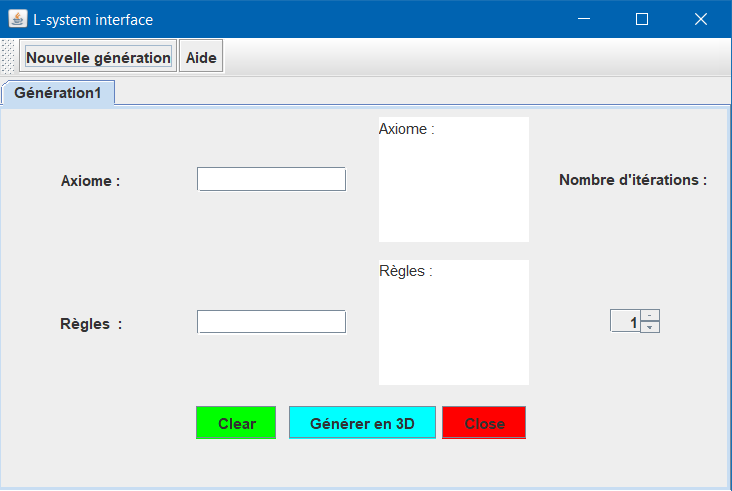
\includegraphics[scale=0.5]{pics/MainFrameGUI.PNG}
    \caption{Fenêtre principale}
    \label{mainframe}
\end{figure}
Il ne vous reste ensuite plus qu'à renseigner votre axiome, ainsi que vos règles et de cliquer sur le bouton \button{Générer en 3D}. Le bouton \button{Close} permet de fermer l'onglet de génération et le bouton \button{Clear} de supprimer votre axiome et vos règles précédemment écrites. Grâce au compteur à droite, vous êtes en mesure de définir le nombre d'itérations de votre génération.

\info{Vous pouvez ouvrir de nouveaux onglets de génération grâce au bouton \button{Nouvelle génération} mais sachez qu'un maximum de trois fenêtres est accepté}

\subsection{Navigation dans l'interface graphique en 3D}
\label{sec:nav_3d}

Pour naviguer dans l'espace 3D, vous pouvez utiliser votre clavier ainsi que votre souris. \info{La souris n'est pas essentielle, elle permet de se déplacer facilement dans l'environnement mais un clavier suffit amplement}

\paragraph{Liste des commandes au clavier : }
\begin{itemize}
    \item \textbf{Z} $\xrightarrow{} Avancer$
    \item \textbf{S} $\xrightarrow{} Reculer$
    \item \textbf{Q} $\xrightarrow{} Aller \ \grave{a} \ gauche$
    \item \textbf{D} $\xrightarrow{} Aller \ \grave{a} \ droite$
    \item \textbf{A} $\xrightarrow{} Tourner \ la \ cam\Acute{e}ra \ \grave{a} \ gauche$
    \item \textbf{E} $\xrightarrow{} Tourner \ la \ cam\Acute{e}ra \ \grave{a} \ droite$
    \item \textbf{W} $\xrightarrow{} Prendre \ de \ la \ hauteur$
    \item \textbf{X} $\xrightarrow{} Perde \ de \ la \ hauteur$
    \end{itemize}
\paragraph{Liste des commandes à la souris :}
    \begin{itemize}
    \item \textbf{Mollette Avant} $\xrightarrow{} Zommer$
    \item \textbf{Mollette Arrière} $\xrightarrow{} D\Acute{e}zoomer$
    \item \textbf{Clic Droit} $\xrightarrow{} Maintenir \ puis \ bouger \ la \ souris \ pour \ changer \ l'orientation \ de \ la \ cam\Acute{e}ra$
    
\end{itemize}

\problem{Vous ne pouvez pas utiliser 2 touches ou plus en même temps pour naviguer. Par exemple, enfoncer les touches \textbf{Z} et \textbf{D} pour aller la direction nord-est  est impossible, il vous faut tourner votre caméra dans la direction où vous voulez aller puis appuyer sur \textbf{Z}.}

Fermez la fenêtre 3D pour pouvoir générer un nouveau L-Système sans avoir à rouvrir l'application

\section{Tests de notre logiciel}

\subsection{Possibles problèmes}

Lorsque vous tentez de générer un L-Système, celui-ci est affiché en 3D en utilisant une méthode récursive, si celui-ci est trop long cela peut entraîner une erreur de type \textit{StackOverflowError}, la fenêtre 3D restera alors blanche. Fermez la puis retentez une génération avec moins d'itérations ou tentez une génération avec d'autres règles.

Si vous lancez une génération avec beaucoup d'itérations, celle-ci peut mettre un certain temps à se générer et peut provoquer une erreur \textit{OutOfMemoryError}.

\section{Mesures de performances}

Nous avons mis en place un stress-test qui réécrit et convertit en arbre le L-Système.
Ce stress-test nécessite 4GB de RAM de libre et construira un mot de quasiment 26 millions de caractères puis celui-ci sera converti en un arbre (notez qu'il est impossible de l'afficher dans le moteur graphique car cela donnera \textit{StackOverflowError}).

\begin{figure}[h!]
    \centering
    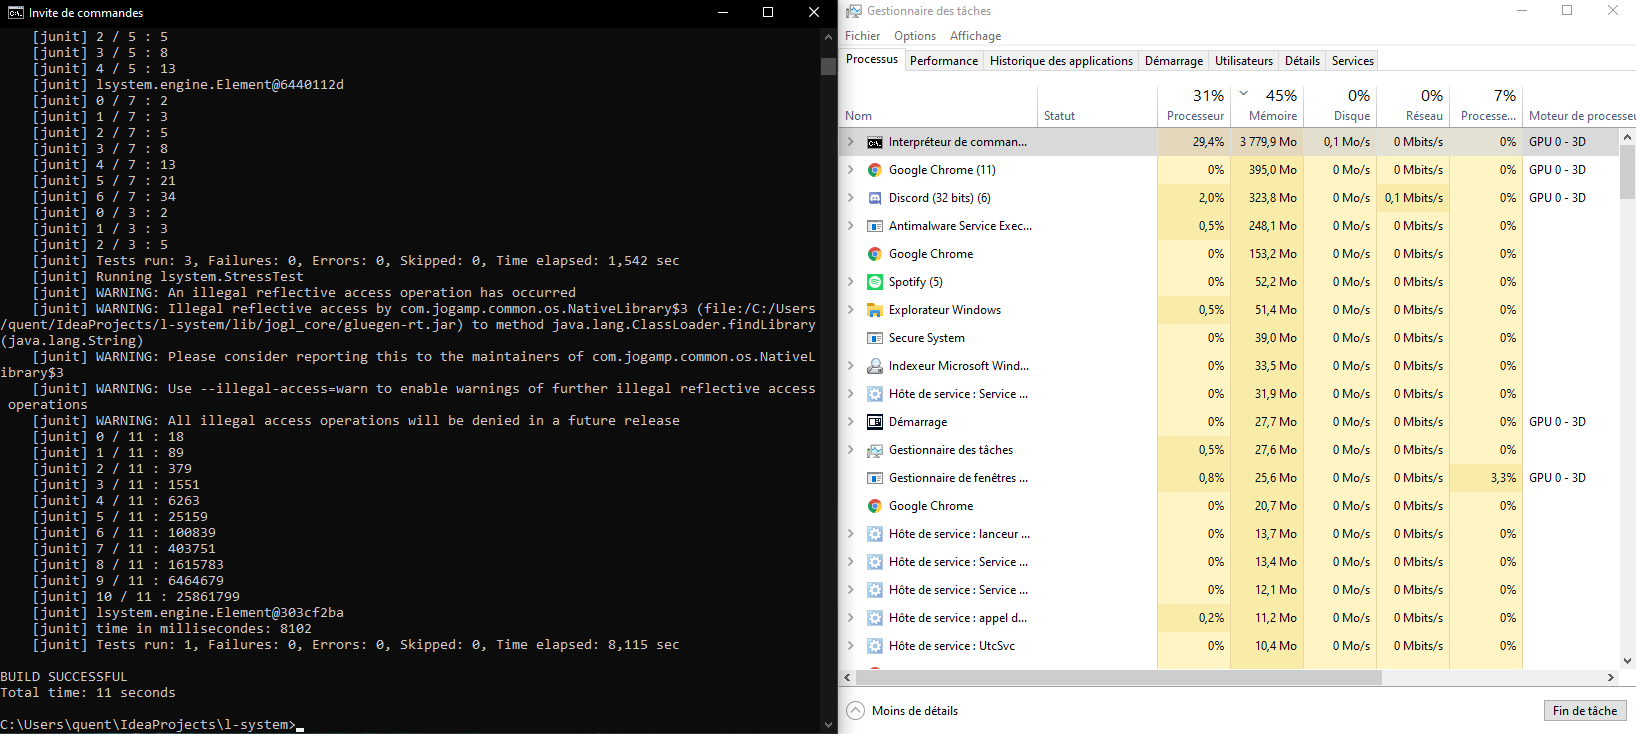
\includegraphics[scale=0.3]{pics/stresstest.png}
    \caption{Mesure de performances}
    \label{Perf}
\end{figure}

(Test de performances effectué avec un Ryzen 5 2400g et une gtx 1050ti.)

\section{Possibles améliorations}

\begin{itemize}
    \item Améliorer l'optimisation.
    \item Rendre l'interface graphique plus conviviale.
    \item Réaliser les L-Système 2D dans un vrai environnement 2D, et non dans un moteur 3D comme actuellement.
    \item Améliorer le réalisme de la modélisation 3D.
    \item Exporter les modèles d'arbres afin de les implémenter facilement dans des applications comme des jeux.
    \item Utilisation des méthodes de OpenGL 3 ou 4 au lieu de ceux de OpenGL 2 afin de profiter des dernières améliorations technologiques des cartes graphiques (notamment au niveau des performances).
    
\end{itemize}
